% ══════════════════════════════════════════════════════════════════════════════
%  ADVANCED ECOSYSTEMS — the above-level book (from 2027)
%  Faculty decision, Nov 2026: every student completes the at-level lesson books;
%  students who excel move on to this book. Its topics go deeper into the ideas
%  of the at-level lessons rather than adding more of the same work.
%
%  Each topic: a reading, the deeper idea worked through (I do / We do), then
%  %%PARTD:N%% pulls in the old Part D questions of at-level Lesson N as
%  practice, then a Challenge. Built by make_a5.py (via a5_levels.py).
% ══════════════════════════════════════════════════════════════════════════════

% ══════════════════════════════════════════════════════════════════════════════
%  TOPIC 1 — CELLS: THE UNITS OF LIFE                        (deepens Lesson 1)
% ══════════════════════════════════════════════════════════════════════════════
\setcounter{section}{0}\renewcommand{\lessonart}{1}
\sectiondiv{Cells: the Units of Life}{Cell theory \textbullet{} Plant and animal cells \textbullet{} Magnification \textbullet{} Why cells are small}\label{sec:1}
\lessoncodes{Deepens Lesson 1 \textbullet{} VC2S8U02 \textbullet{} VC2S8U03}

\vocabhead
\begin{ctab}
\begin{tabular}{|SW{3.4cm}|W{7.0cm}|}
  \hline\hd & \thead{Word} & \thead{Definition (copy from the slide)} \\ \hline
  & \scaf{\textbf{Cell}} & \scaf{The smallest unit that can carry out all the processes of life.} \\ \hline
  & \textbf{Cell theory} & \\ \hline
  & \textbf{Organelle} & \\ \hline
  & \textbf{Nucleus} & \\ \hline
  & \textbf{Chloroplast} & \\ \hline
  & \textbf{Magnification} & \\ \hline
\end{tabular}
\end{ctab}

\lessonpart{A}{Reading and comprehension}{Teal}\label{read:1}

\begin{readingbox}{Reading --- Seeing the Invisible}
In 1665 Robert Hooke looked at a thin slice of cork through one of the first microscopes. He saw rows of tiny empty boxes and called them \emph{cells}, because they reminded him of the small rooms monks lived in. A few years later Antonie van Leeuwenhoek, using lenses he ground himself, saw living ``animalcules'' swimming in pond water: the first people ever to see bacteria and single-celled organisms.

Nearly two hundred years later, scientists put the evidence together into \textbf{cell theory}: every living thing is made of one or more cells; the cell is the smallest unit of life; and every cell comes from a cell that already existed. A bacterium is a single cell. You are about 37 trillion of them, working together.

Inside a cell are smaller parts with their own jobs, called \textbf{organelles}. The \textbf{nucleus} holds the cell's DNA, the instructions for building and running it. Plant cells also have \textbf{chloroplasts}, where light energy is captured to make food.

Most cells are far too small to see. A light microscope makes them look bigger: its \textbf{magnification} tells you how many times bigger the image is than the real thing.
\end{readingbox}

\rcreset
\rcq{What did Hooke see in cork, and why did he call them cells?}{2.5cm}
\rcq{State the three ideas of cell theory.}{3cm}
\rcq{What is an organelle? Give two examples and their jobs.}{2.5cm}
\rcq{Why could nobody study cells before the 1600s?}{2cm}

\lessonpart{B}{Theory and examples}{Blue}\label{theory:1}

\subsection{Plant and Animal Cells}\label{sub:a1.1}

\begin{ctab}
\begin{tabular}{|C{3.0cm}|C{1.5cm}|C{1.5cm}|W{4.0cm}|}
  \hline\thead{Part} & \thead{Animal} & \thead{Plant} & \thead{Job} \\ \hline
  Cell membrane & yes & yes & controls what enters and leaves \\ \hline
  Cytoplasm & yes & yes & jelly where most reactions happen \\ \hline
  Nucleus & yes & yes & holds the DNA; controls the cell \\ \hline
  Mitochondria & yes & yes & release energy from food (respiration) \\ \hline
  Cell wall & no & yes & stiff outer layer that supports the cell \\ \hline
  Chloroplasts & no & yes & capture light to make food (photosynthesis) \\ \hline
  Large vacuole & no & yes & stores water and keeps the cell firm \\ \hline
\end{tabular}
\end{ctab}

\begin{workedex}{Plant or animal?}
A cell from a leaf of a pondweed has a nucleus, a cell wall, a large vacuole and many small green discs.

\smallskip
It is a \textbf{plant} cell. The cell wall and large vacuole are found only in plant cells, and the green discs are chloroplasts, which make food by photosynthesis.
\end{workedex}

\begin{wedo}{Plant or animal?}
A cell scraped from the inside of a cheek has a nucleus, a cell membrane and cytoplasm, but no cell wall and no chloroplasts. A cell from an onion bulb has a cell wall and a large vacuole but no chloroplasts. Identify each cell, and explain why the onion cell has no chloroplasts even though it is a plant cell.
\answerbox{5cm}
\end{wedo}

\subsection{Magnification}\label{sub:a1.2}

\begin{skillbox}{Magnification}
\[ \text{magnification} = \frac{\text{image size}}{\text{actual size}} \]
Both sizes must be in the same unit. Cells are measured in micrometres (\textmu m): $1\,\text{mm} = 1000\,\text{\textmu m}$.
\end{skillbox}

\begin{workedex}{Finding the magnification}
A cheek cell is 60\,\textmu m across. In a photograph it measures 30\,mm. Find the magnification.

\smallskip
Same units first: $30\,\text{mm} = 30 \times 1000 = 30\,000\,\text{\textmu m}$.\\
Magnification $= 30\,000 \div 60 = \mathbf{500\times}$.
\end{workedex}

\begin{wedo}{Finding the actual size}
A photograph of a red blood cell taken at $\times 2000$ shows the cell as 16\,mm across. Find the actual width of the cell in micrometres. (Rearrange: actual size $=$ image size $\div$ magnification.)
\workbox{4.5cm}
\end{wedo}

\lessonpart{C}{Practice}{Amber}\label{prac:1}

%%PARTD:1%%

\needspace{10\baselineskip}
\task A leaf cell is 0.1\,mm long. Calculate how long it would appear under a microscope set to $\times 400$, in millimetres.
\workbox{4cm}

\lessonpart{D}{Challenge}{Violet}\label{ext:1}

\task Why are cells so small? A cell takes in food and oxygen through its surface, but uses them throughout its volume.
\pt{a} Calculate the surface area and the volume of a cube of side 1\,cm and a cube of side 3\,cm, and the surface area to volume ratio of each.
\workbox{6cm}
\pt{b} Use your answers to explain why a large organism is made of many small cells instead of one huge cell.
\answerbox{5cm}

\clearpage

% ══════════════════════════════════════════════════════════════════════════════
%  TOPIC 2 — THE TREE OF LIFE: DOMAINS AND DNA          (deepens Lessons 2, 3)
% ══════════════════════════════════════════════════════════════════════════════
\setcounter{section}{1}\renewcommand{\lessonart}{2}
\sectiondiv{The Tree of Life: Domains and DNA}{Three domains \textbullet{} Prokaryotes and eukaryotes \textbullet{} Reading an evolutionary tree \textbullet{} DNA evidence}\label{sec:2}
\lessoncodes{Deepens Lessons 2 and 3 \textbullet{} VC2S8U01 \textbullet{} VC2S10U04 \textbullet{} VC2S10U05}

\vocabhead
\begin{ctab}
\begin{tabular}{|SW{3.4cm}|W{7.0cm}|}
  \hline\hd & \thead{Word} & \thead{Definition (copy from the slide)} \\ \hline
  & \scaf{\textbf{Domain}} & \scaf{The largest group in classification, above kingdom. There are three: Bacteria, Archaea and Eukarya.} \\ \hline
  & \textbf{Prokaryote} & \\ \hline
  & \textbf{Eukaryote} & \\ \hline
  & \textbf{Common ancestor} & \\ \hline
  & \textbf{Evolutionary tree} & \\ \hline
  & \textbf{DNA sequence} & \\ \hline
\end{tabular}
\end{ctab}

\lessonpart{A}{Reading and comprehension}{Teal}\label{read:2}

\begin{readingbox}{Reading --- The Microbes That Rewrote the Tree}
For most of the 1900s, scientists sorted every tiny single-celled organism without a nucleus into one group: bacteria. Cells like these, with their DNA loose in the cytoplasm, are \textbf{prokaryotes}. Cells with a nucleus, like ours, are \textbf{eukaryotes}.

In 1977 the American scientist Carl Woese compared not what microbes looked like, but the order of the chemical ``letters'' in one of their genes: their \textbf{DNA sequence}. Some microbes from hot springs and salty lakes turned out to be as different from bacteria, in their genes, as bacteria are from us. Woese named them Archaea and proposed a new top level of classification: three \textbf{domains}, Bacteria, Archaea and Eukarya. Many scientists thought he was wrong. Today his three domains are in every textbook.

DNA changes slowly over many generations. Two species that split from a \textbf{common ancestor} recently have had little time to build up differences, so their DNA is very alike. Species that split long ago differ more. Scientists use these differences to draw an \textbf{evolutionary tree}: a diagram showing which groups share the most recent ancestors.
\end{readingbox}

\rcreset
\rcq{What is the difference between a prokaryote and a eukaryote?}{2.5cm}
\rcq{What evidence did Woese use, and why was it new?}{2.5cm}
\rcq{Why were many scientists slow to accept the three domains? What made them change their minds?}{3cm}
\rcq{Why do closely related species have very similar DNA?}{2.5cm}

\lessonpart{B}{Theory and examples}{Blue}\label{theory:2}

\subsection{Three Domains}\label{sub:a2.1}

\begin{ctab}
\begin{tabular}{|C{2.3cm}|W{2.6cm}|W{5.3cm}|}
  \hline\thead{Domain} & \thead{Cell type} & \thead{Examples} \\ \hline
  Bacteria & prokaryote & \textit{E.\ coli}, the bacteria in yoghurt and in soil \\ \hline
  Archaea & prokaryote & microbes of hot springs, salt lakes and animal guts \\ \hline
  Eukarya & eukaryote & every protist, fungus, plant and animal \\ \hline
\end{tabular}
\end{ctab}

\begin{workedex}{Placing an organism}
A microbe found in the salt lakes of the Victorian Mallee has no nucleus, and its genes are unlike those of any bacterium.

\smallskip
No nucleus means it is a prokaryote, so it is in Bacteria or Archaea. Its genes are unlike any bacterium's, so it belongs in \textbf{Archaea}. Its home, a salty lake, is typical of archaea, but the genes are the deciding evidence.
\end{workedex}

\begin{wedo}{Placing an organism}
Place each in a domain and give your reason: a mushroom; the bacterium that turns milk into yoghurt; a single-celled algae with a nucleus and a chloroplast.
\answerbox{4.5cm}
\end{wedo}

\subsection{Reading an Evolutionary Tree}\label{sub:a2.2}

\begin{center}
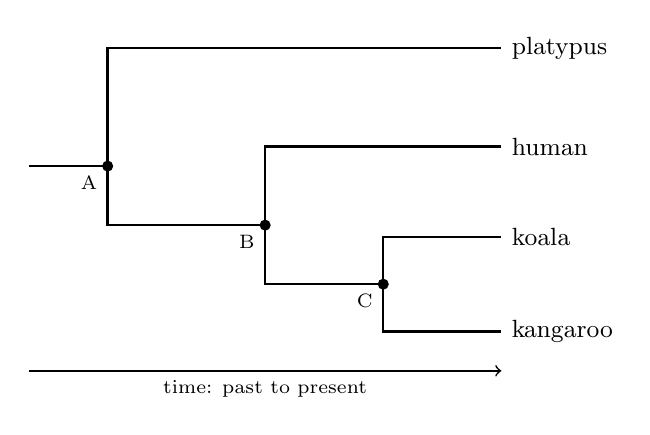
\begin{tikzpicture}[font=\small, line width=0.9pt]
  \draw (0,0) -- (1,0);
  \draw (1,0) -- (1,1.5) -- (6,1.5) node[right] {platypus};
  \draw (1,0) -- (1,-0.75) -- (3,-0.75);
  \draw (3,-0.75) -- (3,0.25) -- (6,0.25) node[right] {human};
  \draw (3,-0.75) -- (3,-1.5) -- (4.5,-1.5);
  \draw (4.5,-1.5) -- (4.5,-0.9) -- (6,-0.9) node[right] {koala};
  \draw (4.5,-1.5) -- (4.5,-2.1) -- (6,-2.1) node[right] {kangaroo};
  \fill (1,0) circle (2pt) (3,-0.75) circle (2pt) (4.5,-1.5) circle (2pt);
  \node[below left, font=\scriptsize] at (1,0) {A};
  \node[below left, font=\scriptsize] at (3,-0.75) {B};
  \node[below left, font=\scriptsize] at (4.5,-1.5) {C};
  \draw[->, line width=0.6pt] (0,-2.6) -- (6,-2.6) node[midway, below, font=\scriptsize] {time: past to present};
\end{tikzpicture}
\figcap{Each dot is a common ancestor. The later two groups split, the more closely they are related.}
\end{center}

\begin{workedex}{Who is more closely related?}
Is the koala more closely related to the kangaroo or to the human?

\smallskip
The koala and kangaroo share ancestor C. The koala and human only share ancestor B, which lived earlier. So the koala is \textbf{more closely related to the kangaroo}: they split from each other more recently.
\end{workedex}

\begin{wedo}{Who is more closely related?}
Use the tree. Is the human more closely related to the kangaroo or to the platypus? Which ancestor do all four share?
\answerbox{4cm}
\end{wedo}

\lessonpart{C}{Practice}{Amber}\label{prac:2}

%%PARTD:2%%

%%PARTD:3%%

\lessonpart{D}{Challenge}{Violet}\label{ext:2}

\task Scientists compared 100 letters of the same gene in four species, W, X, Y and Z. The table shows how many letters differ between each pair.
\begin{ctab}
\begin{tabular}{|C{1.4cm}|C{1.4cm}|C{1.4cm}|C{1.4cm}|C{1.4cm}|}
  \hline & \thead{W} & \thead{X} & \thead{Y} & \thead{Z} \\ \hline
  \thead{W} & --- & 3 & 11 & 19 \\ \hline
  \thead{X} & 3 & --- & 12 & 19 \\ \hline
  \thead{Y} & 11 & 12 & --- & 20 \\ \hline
  \thead{Z} & 19 & 19 & 20 & --- \\ \hline
\end{tabular}
\end{ctab}
\pt{a} Which two species are most closely related? Which species split off from the others first?
\answerbox{3cm}
\pt{b} Draw an evolutionary tree for the four species, like the one in Part B.
\drawbox{6cm}{}

\clearpage

% ══════════════════════════════════════════════════════════════════════════════
%  TOPIC 3 — WHAT IS A SPECIES? KEYS AND DNA BARCODES        (deepens Lesson 4)
% ══════════════════════════════════════════════════════════════════════════════
\setcounter{section}{2}\renewcommand{\lessonart}{4}
\sectiondiv{What Is a Species? Keys and DNA Barcodes}{Defining a species \textbullet{} Hybrids \textbullet{} Writing a key that works \textbullet{} DNA barcoding}\label{sec:3}
\lessoncodes{Deepens Lesson 4 \textbullet{} VC2S8U01 \textbullet{} VC2S10I06}

\vocabhead
\begin{ctab}
\begin{tabular}{|SW{3.4cm}|W{7.0cm}|}
  \hline\hd & \thead{Word} & \thead{Definition (copy from the slide)} \\ \hline
  & \scaf{\textbf{Fertile}} & \scaf{Able to produce young of its own.} \\ \hline
  & \textbf{Hybrid} & \\ \hline
  & \textbf{Cryptic species} & \\ \hline
  & \textbf{Couplet} & \\ \hline
  & \textbf{DNA barcode} & \\ \hline
\end{tabular}
\end{ctab}

\lessonpart{A}{Reading and comprehension}{Teal}\label{read:3}

\begin{readingbox}{Reading --- One Species or Two?}
The usual definition says a species is a group of organisms that can breed together and have \textbf{fertile} young. It works well for most animals. A horse and a donkey can breed, but their young, a mule, is almost always sterile, so horses and donkeys are separate species. A mule is a \textbf{hybrid}: the young of two different species.

But the definition has problems. Bacteria do not breed in pairs at all. Fossils cannot be tested for breeding. Some plants form fertile hybrids easily. And some animals look identical but never breed together: they are \textbf{cryptic species}, hidden from anyone who only looks. Frogs that look the same but have different calls are a common example.

Because of this, scientists now use several lines of evidence together: appearance, behaviour, where the organism lives, and its DNA. A short, standard stretch of an animal's DNA can work like the barcode on a packet in a supermarket. Comparing this \textbf{DNA barcode} against a library of known species can name an organism from a single hair, a scale or a scrap of leaf.
\end{readingbox}

\rcreset
\rcq{Why are horses and donkeys separate species, even though they can breed?}{2.5cm}
\rcq{Give two kinds of organism the breeding definition does not work for, and why.}{3cm}
\rcq{What is a cryptic species, and how might scientists discover one?}{2.5cm}
\rcq{Why can a DNA barcode identify an organism a key cannot?}{2.5cm}

\lessonpart{B}{Theory and examples}{Blue}\label{theory:3}

\subsection{Writing a Key That Works}\label{sub:a3.1}

\begin{skillbox}{Rules for a good couplet}
Each step of a key is a \textbf{couplet}: two statements, and every organism must fit exactly one.
\textbf{1.} Use features anyone can see on any adult of the species. \textbf{2.} Make the two halves opposites (``has a pouch'' / ``has no pouch''). \textbf{3.} Avoid size, colour and ``big or small'', which vary between individuals. \textbf{4.} Split the group, roughly in half if you can.
\end{skillbox}

\begin{workedex}{Fixing a weak couplet}
\textbf{Weak:} 1a.\ Large brown bird \qquad 1b.\ Small bird with a long tail

\smallskip
``Large'' and ``small'' depend on what you compare them with, a young bird may be small, and the two halves describe different features (colour, tail), so a small brown bird with a short tail fits neither.
\textbf{Better:} 1a.\ Tail longer than body \qquad 1b.\ Tail shorter than body.
\end{workedex}

\begin{wedo}{Fixing a weak couplet}
Rewrite this couplet so it follows all four rules: 2a.\ Green frog with spots \qquad 2b.\ Brown frog that is good at climbing.
\answerbox{4cm}
\end{wedo}

\subsection{Is It a Separate Species?}\label{sub:a3.2}

\begin{workedex}{Using several lines of evidence}
Two populations of tree frog in eastern Victoria look the same. Females only move towards the call of their own population, and their DNA barcodes differ by 6\%. (Individuals of one species usually differ by less than 2\%.)

\smallskip
They do not breed together, because the females choose different calls, and their DNA is far more different than within one species. Both lines of evidence say they are \textbf{two cryptic species}.
\end{workedex}

\begin{wedo}{Using several lines of evidence}
Lions and tigers do not meet in the wild. In zoos they can breed, and their young (ligers) are usually sterile. Decide whether lions and tigers are one species or two, and use two lines of evidence.
\answerbox{4.5cm}
\end{wedo}

\lessonpart{C}{Practice}{Amber}\label{prac:3}

%%PARTD:4%%

\lessonpart{D}{Challenge}{Violet}\label{ext:3}

\task Write a dichotomous key that identifies these six Australian animals. Use only features in the table, follow the four rules, and use five couplets.
\begin{ctab}
\begin{tabular}{|W{2.5cm}|C{1.6cm}|C{1.5cm}|C{1.5cm}|C{1.5cm}|}
  \hline\thead{Animal} & \thead{Body covering} & \thead{Lays eggs} & \thead{Pouch} & \thead{Wings} \\ \hline
  Platypus & fur & yes & no & no \\ \hline
  Echidna & fur and spines & yes & yes & no \\ \hline
  Koala & fur & no & yes & no \\ \hline
  Dingo & fur & no & no & no \\ \hline
  Kookaburra & feathers & yes & no & yes \\ \hline
  Blue-tongue lizard & scales & no & no & no \\ \hline
\end{tabular}
\end{ctab}
\answerbox{8cm}

\clearpage

% ══════════════════════════════════════════════════════════════════════════════
%  TOPIC 4 — MEASURING BIODIVERSITY                          (deepens Lesson 5)
% ══════════════════════════════════════════════════════════════════════════════
\setcounter{section}{3}\renewcommand{\lessonart}{5}
\sectiondiv{Measuring Biodiversity}{Sampling \textbullet{} Richness and evenness \textbullet{} Simpson's index \textbullet{} Capture--recapture}\label{sec:4}
\lessoncodes{Deepens Lesson 5 \textbullet{} VC2S8U04 \textbullet{} VC2S10I03 \textbullet{} VC2S10I04}

\vocabhead
\begin{ctab}
\begin{tabular}{|SW{3.4cm}|W{7.0cm}|}
  \hline\hd & \thead{Word} & \thead{Definition (copy from the slide)} \\ \hline
  & \scaf{\textbf{Sample}} & \scaf{A small part of an area or population, studied to estimate what the whole is like.} \\ \hline
  & \textbf{Species richness} & \\ \hline
  & \textbf{Species evenness} & \\ \hline
  & \textbf{Diversity index} & \\ \hline
  & \textbf{Capture--recapture} & \\ \hline
\end{tabular}
\end{ctab}

\lessonpart{A}{Reading and comprehension}{Teal}\label{read:4}

\begin{readingbox}{Reading --- Counting What You Cannot See}
How many skinks live in a grassland? Nobody can find every one. Ecologists study a \textbf{sample} instead: a few quadrats, a line of pitfall traps, or a set of camera traps, chosen so they represent the whole area. Then they scale up.

Counting species is only half the story. \textbf{Species richness} is the number of species. \textbf{Species evenness} is how equal their numbers are. Imagine two paddocks, each with four plant species and 100 plants. In the first, there are 25 of each. In the second, there are 97 of one weed and one each of the others. They have the same richness, but the first is far more diverse, because no single species dominates.

A \textbf{diversity index} combines richness and evenness into one number, so places can be compared fairly. For animals that move, ecologists use \textbf{capture--recapture}: they catch some animals, mark them harmlessly, release them, then catch again later. The share of marked animals in the second catch reveals how big the whole population is.
\end{readingbox}

\rcreset
\rcq{Why do ecologists sample instead of counting every organism?}{2.5cm}
\rcq{Explain the difference between species richness and species evenness.}{2.5cm}
\rcq{Which of the two paddocks in the reading has higher biodiversity, and why?}{2.5cm}
\rcq{Why must a sample be chosen to represent the whole area?}{2.5cm}

\lessonpart{B}{Theory and examples}{Blue}\label{theory:4}

\subsection{Simpson's Diversity Index}\label{sub:a4.1}

\begin{skillbox}{Simpson's index}
\[ D = 1 - \sum\left(\frac{n}{N}\right)^2 \]
$n$ is the number of one species, $N$ the total of all organisms. Work out $\frac{n}{N}$ for every species, square each one, add them up, and take the total away from 1. $D$ runs from 0 (one species only) towards 1 (many species, evenly spread).
\end{skillbox}

\begin{workedex}{Calculating $D$}
A quadrat holds 20 plants: 6 wallaby grass, 6 kangaroo grass, 6 daisies and 2 orchids.

\smallskip
$\frac{n}{N}$: $\ 0.3,\ 0.3,\ 0.3,\ 0.1$ \quad squared: $\ 0.09,\ 0.09,\ 0.09,\ 0.01$\\
Sum $= 0.28$, so $D = 1 - 0.28 = \mathbf{0.72}$: a fairly diverse quadrat.
\end{workedex}

\begin{wedo}{Calculating $D$}
A quadrat holds 20 plants: 8 of species P, 8 of species Q and 4 of species R. Calculate $D$, and say whether it is more or less diverse than the worked example.
\workbox{5cm}
\end{wedo}

\subsection{Capture--Recapture}\label{sub:a4.2}

\begin{skillbox}{Estimating a population}
\[ \text{population} \approx \frac{\text{number marked} \times \text{number caught second time}}{\text{number of marked animals recaught}} \]
It assumes marks do not fall off or harm the animal, marked animals mix back in, and no animals are born, die or move in between the two catches.
\end{skillbox}

\begin{workedex}{Estimating a population}
Ecologists catch and mark 30 skinks. A week later they catch 40, and 8 of them are marked.

\smallskip
Population $\approx \dfrac{30 \times 40}{8} = \dfrac{1200}{8} = \mathbf{150}$ skinks.
\end{workedex}

\begin{wedo}{Estimating a population}
Rangers mark 20 eastern barred bandicoots. Two weeks later they trap 25, and 5 are marked. Estimate the population, and give one reason the estimate could be wrong.
\workbox{5cm}
\end{wedo}

\lessonpart{C}{Practice}{Amber}\label{prac:4}

%%PARTD:5%%

\needspace{10\baselineskip}
\task Ten 1\,m$^2$ quadrats in a 2000\,m$^2$ grassland hold 3, 5, 2, 4, 0, 6, 3, 4, 5 and 2 orchids. Estimate the number of orchids in the whole grassland. Show your working.
\workbox{5cm}

\lessonpart{D}{Challenge}{Violet}\label{ext:4}

\task In a capture--recapture study, the marked animals learn that the traps hold food, and walk into them more readily the second time.
\pt{a} Will the number of marked animals recaught be too high or too low? Explain.
\answerbox{3.5cm}
\pt{b} Will the population estimate be too high or too low? Use the formula to explain.
\answerbox{3.5cm}
\pt{c} Suggest a change to the method that would reduce the problem.
\answerbox{3cm}

\clearpage

% ══════════════════════════════════════════════════════════════════════════════
%  TOPIC 5 — ENERGY FLOW AND THE CARBON CYCLE           (deepens Lessons 6, 7)
% ══════════════════════════════════════════════════════════════════════════════
\setcounter{section}{4}\renewcommand{\lessonart}{6}
\sectiondiv{Energy Flow and the Carbon Cycle}{Where the energy goes \textbullet{} Pyramids of energy \textbullet{} Photosynthesis and respiration \textbullet{} Tipping points}\label{sec:5}
\lessoncodes{Deepens Lessons 6 and 7 \textbullet{} VC2S8U04 \textbullet{} VC2S10U10}

\vocabhead
\begin{ctab}
\begin{tabular}{|SW{3.4cm}|W{7.0cm}|}
  \hline\hd & \thead{Word} & \thead{Definition (copy from the slide)} \\ \hline
  & \scaf{\textbf{Trophic level}} & \scaf{A feeding level in a food chain: producers, primary consumers, secondary consumers, and so on.} \\ \hline
  & \textbf{Pyramid of energy} & \\ \hline
  & \textbf{Photosynthesis} & \\ \hline
  & \textbf{Respiration} & \\ \hline
  & \textbf{Carbon cycle} & \\ \hline
  & \textbf{Tipping point} & \\ \hline
\end{tabular}
\end{ctab}

\lessonpart{A}{Reading and comprehension}{Teal}\label{read:5}

\begin{readingbox}{Reading --- Where Does the Energy Go?}
A wedge-tailed eagle eats rabbits; the rabbits eat grass. Yet in any grassland there is far more grass than rabbits, and far more rabbits than eagles. The reason is energy. Each feeding level, or \textbf{trophic level}, passes on only about one-tenth of the energy it takes in. Most of the rest is used to stay alive and released as heat during \textbf{respiration}; some is in parts that are never eaten, such as roots and bones, and some passes out as waste. Drawn as stacked bars, the energy at each level makes a \textbf{pyramid of energy}.

Energy flows through an ecosystem in one direction and is lost as heat. Matter is different: it is recycled. Carbon is taken from the air as carbon dioxide during \textbf{photosynthesis}, built into the plant, passed along food chains, and returned to the air by respiration, decomposition and fire. This loop is the \textbf{carbon cycle}.

Ecosystems can absorb a lot of damage and recover. But past a \textbf{tipping point}, an ecosystem flips into a different, poorer state and stays there. Mountain ash trees take about twenty years to produce seed. If two fires burn a forest within twenty years, the young trees die before they can seed, and the forest can turn permanently into scrub.
\end{readingbox}

\rcreset
\rcq{Give three reasons most of the energy at one trophic level does not reach the next.}{3cm}
\rcq{Why are there fewer eagles than rabbits in a grassland?}{2.5cm}
\rcq{How is the way carbon moves through an ecosystem different from the way energy moves?}{3cm}
\rcq{Explain why two fires close together can destroy a mountain ash forest for good.}{2.5cm}

\lessonpart{B}{Theory and examples}{Blue}\label{theory:5}

\subsection{Pyramids of Energy}\label{sub:a5.1}

\begin{center}
\begin{tikzpicture}[font=\small]
  \draw[Ink, line width=0.8pt, fill=black!8] (-3,0) rectangle (3,0.7);
  \draw[Ink, line width=0.8pt, fill=black!8] (-1.6,0.7) rectangle (1.6,1.4);
  \draw[Ink, line width=0.8pt, fill=black!8] (-0.8,1.4) rectangle (0.8,2.1);
  \draw[Ink, line width=0.8pt, fill=black!8] (-0.35,2.1) rectangle (0.35,2.8);
  \node at (0,0.35) {producers 20\,000\,kJ};
  \node at (0,1.05) {2000\,kJ};
  \node at (0,1.75) {200};
  \node at (0,2.45) {20};
  \node[right, font=\scriptsize] at (3.2,0.35) {grass};
  \node[right, font=\scriptsize] at (3.2,1.05) {rabbit (primary)};
  \node[right, font=\scriptsize] at (3.2,1.75) {fox (secondary)};
  \node[right, font=\scriptsize] at (3.2,2.45) {eagle (tertiary)};
\end{tikzpicture}
\figcap{About 10\% of the energy passes up each level. (Bars not to scale.)}
\end{center}

\begin{workedex}{Why food chains are short}
Using the pyramid, what share of the grass's energy reaches the eagle?

\smallskip
$20 \div 20\,000 = 0.001$, so only \textbf{0.1\%}. A fifth level would get about 2\,kJ, far too little to support a population. That is why food chains rarely have more than four or five links.
\end{workedex}

\begin{wedo}{Why food chains are short}
The producers in a wetland hold 50\,000\,kJ. Calculate the energy reaching each of the next three levels, and the percentage of the producers' energy that reaches the third consumer.
\workbox{5cm}
\end{wedo}

\subsection{Carbon In and Out}\label{sub:a5.2}

\begin{skillbox}{Two word equations}
\textbf{Photosynthesis} (in chloroplasts, needs light):\quad carbon dioxide $+$ water $\rightarrow$ glucose $+$ oxygen\\
\textbf{Respiration} (in every living cell):\quad glucose $+$ oxygen $\rightarrow$ carbon dioxide $+$ water $+$ energy
\end{skillbox}

\begin{workedex}{Tracing a carbon atom}
A carbon atom in the air ends up in a kangaroo and then back in the air. Describe its path.

\smallskip
Grass takes in the carbon dioxide and, by photosynthesis, builds the carbon into glucose and then into its leaves. A kangaroo eats the grass and builds the carbon into its own body. When the kangaroo's cells use the glucose in respiration, or when the kangaroo dies and decomposers respire, the carbon is released into the air again as carbon dioxide.
\end{workedex}

\begin{wedo}{Tracing a carbon atom}
Describe the path of a carbon atom from the air into a eucalyptus leaf, and back into the air when the leaf is burnt in a bushfire. Name the processes.
\answerbox{5cm}
\end{wedo}

\lessonpart{C}{Practice}{Amber}\label{prac:5}

%%PARTD:6%%

%%PARTD:7%%

\lessonpart{D}{Challenge}{Violet}\label{ext:5}

\task A mountain ash forest stores a great deal of carbon in its trees. Explain, using the carbon cycle and the idea of a tipping point, how logging followed by a bushfire within twenty years could change the forest, and what that would do to the amount of carbon dioxide in the air.
\answerbox{8cm}

\clearpage

% ══════════════════════════════════════════════════════════════════════════════
%  TOPIC 6 — NATURAL SELECTION AND EVOLUTION                 (deepens Lesson 8)
% ══════════════════════════════════════════════════════════════════════════════
\setcounter{section}{5}\renewcommand{\lessonart}{8}
\sectiondiv{Natural Selection and Evolution}{Variation and selection \textbullet{} Evolution we can watch \textbullet{} Similar bodies, different reasons}\label{sec:6}
\lessoncodes{Deepens Lesson 8 \textbullet{} VC2S8U04 \textbullet{} VC2S10U05}

\vocabhead
\begin{ctab}
\begin{tabular}{|SW{3.4cm}|W{7.0cm}|}
  \hline\hd & \thead{Word} & \thead{Definition (copy from the slide)} \\ \hline
  & \scaf{\textbf{Variation}} & \scaf{The differences between individuals of the same species.} \\ \hline
  & \textbf{Natural selection} & \\ \hline
  & \textbf{Evolution} & \\ \hline
  & \textbf{Mutation} & \\ \hline
  & \textbf{Homologous structures} & \\ \hline
  & \textbf{Convergent evolution} & \\ \hline
\end{tabular}
\end{ctab}

\lessonpart{A}{Reading and comprehension}{Teal}\label{read:6}

\begin{readingbox}{Reading --- Toads on the Move}
Cane toads were released in Queensland in 1935 and have been spreading west ever since. In the 2000s, scientists measured toads along the invasion front in the Northern Territory and found something surprising: the toads at the very front had longer legs than toads in older populations, and they were moving faster every year. The species was changing before the scientists' eyes.

The explanation is \textbf{natural selection}. Toads vary: some are born with slightly longer legs than others. This \textbf{variation} comes from small, random changes in DNA called \textbf{mutations}, and from the way parents' genes are mixed. Long-legged toads travel further, so they reach new land first, where there is plenty of food and no competition, and breed there. Their young inherit long legs. At the front, long-leggedness is selected, generation after generation.

Change in a species over many generations like this is \textbf{evolution}. Charles Darwin and Alfred Russel Wallace proposed it in 1858. It explains why living things are suited to their environments, and why related species share the same body plan.
\end{readingbox}

\rcreset
\rcq{What did scientists notice about toads at the invasion front?}{2.5cm}
\rcq{Where does variation between individuals come from?}{2.5cm}
\rcq{Explain why long-legged toads leave more young at the front.}{3cm}
\rcq{Did any single toad's legs grow longer during its life? Explain.}{2.5cm}

\lessonpart{B}{Theory and examples}{Blue}\label{theory:6}

\subsection{Natural Selection, Step by Step}\label{sub:a6.1}

\begin{skillbox}{The four steps}
\textbf{Variation:} individuals differ. \quad \textbf{Inheritance:} some differences are passed to the young. \quad \textbf{Selection:} individuals with helpful features survive and breed more. \quad \textbf{Time:} over many generations, the helpful feature becomes common.
\end{skillbox}

\begin{workedex}{Rabbits and myxoma}
When myxoma virus was released in 1950, it killed over 99\% of infected rabbits. Within a few decades most wild rabbits survived it. Why?

\smallskip
\textbf{Variation:} a few rabbits had genes that made them resist the virus. \textbf{Selection:} they survived while others died. \textbf{Inheritance:} their young inherited the resistance. \textbf{Time:} over many generations, resistant rabbits became most of the population.
\end{workedex}

\begin{wedo}{Antibiotic resistance}
A patient stops taking antibiotics as soon as they feel better, and a few bacteria survive. Use the four steps to explain how this can lead to an infection the antibiotic no longer cures.
\answerbox{5cm}
\end{wedo}

\subsection{Similar Bodies, Different Reasons}\label{sub:a6.2}

\begin{workedex}{Homologous structures}
A human arm, a bat wing, a whale flipper and a kangaroo's front leg look different and do different jobs, but they have the same set of bones in the same order.

\smallskip
They are \textbf{homologous structures}: the same body plan, inherited from a shared ancestor and changed by natural selection for different uses. They are evidence that these mammals are related.
\end{workedex}

\begin{wedo}{Same job, different ancestors}
A bird's wing and a bee's wing both let the animal fly, but are built from completely different parts. Explain why these wings are \emph{not} evidence that birds and bees are closely related.
\answerbox{4.5cm}
\end{wedo}

\lessonpart{C}{Practice}{Amber}\label{prac:6}

%%PARTD:8%%

\lessonpart{D}{Challenge}{Violet}\label{ext:6}

\task A student writes: ``Giraffes stretched their necks to reach high leaves, so their babies were born with longer necks.''
\pt{a} Explain what is wrong with this explanation.
\answerbox{4cm}
\pt{b} Rewrite it correctly, using all four steps of natural selection.
\answerbox{5.5cm}

\clearpage

% ══════════════════════════════════════════════════════════════════════════════
%  TOPIC 7 — POPULATIONS, INVADERS AND EXTINCTION   (deepens Lessons 9, 10, 11)
% ══════════════════════════════════════════════════════════════════════════════
\setcounter{section}{6}\renewcommand{\lessonart}{9}
\sectiondiv{Populations, Invaders and Extinction}{Population growth \textbullet{} Carrying capacity \textbullet{} Why small populations are fragile \textbullet{} Genetic rescue}\label{sec:7}
\lessoncodes{Deepens Lessons 9, 10 and 11 \textbullet{} VC2S8U04 \textbullet{} VC2S10H03}

\vocabhead
\begin{ctab}
\begin{tabular}{|SW{3.4cm}|W{7.0cm}|}
  \hline\hd & \thead{Word} & \thead{Definition (copy from the slide)} \\ \hline
  & \scaf{\textbf{Population}} & \scaf{All the individuals of one species living in an area.} \\ \hline
  & \textbf{Exponential growth} & \\ \hline
  & \textbf{Carrying capacity} & \\ \hline
  & \textbf{Limiting factor} & \\ \hline
  & \textbf{Inbreeding} & \\ \hline
  & \textbf{Genetic rescue} & \\ \hline
\end{tabular}
\end{ctab}

\lessonpart{A}{Reading and comprehension}{Teal}\label{read:7}

\begin{readingbox}{Reading --- Twenty-Four Rabbits}
In 1859 about two dozen rabbits were released on a property near Geelong. With plenty of grass and few predators, each pair could raise dozens of young a year. Within seventy years there were hundreds of millions of rabbits across Australia. When nothing holds a population back, it keeps doubling: this is \textbf{exponential growth}.

No population can grow forever. Sooner or later food, water, shelter, predators or disease hold it back. These are \textbf{limiting factors}. The largest population an area can support for a long time is its \textbf{carrying capacity}. A population usually grows quickly, then levels off near the carrying capacity.

Small populations face the opposite danger. When only a few animals are left, relatives breed with each other. This \textbf{inbreeding} reduces genetic diversity and makes harmful features more common, so fewer young survive and the population shrinks further. In the 2010s, the mountain pygmy possums at Mt Buller were inbred and declining. Scientists brought in a few males from Mt Hotham. Their young were larger and survived better, and the population grew. This is \textbf{genetic rescue}.
\end{readingbox}

\rcreset
\rcq{Why did the rabbit population grow so fast after 1859?}{2.5cm}
\rcq{Name four limiting factors.}{2cm}
\rcq{What is the carrying capacity of an area?}{2cm}
\rcq{Explain how inbreeding can make a small population smaller still.}{3cm}
\rcq{How did bringing in males from Mt Hotham help the Mt Buller possums?}{2.5cm}

\lessonpart{B}{Theory and examples}{Blue}\label{theory:7}

\subsection{Two Kinds of Growth}\label{sub:a7.1}

\begin{center}
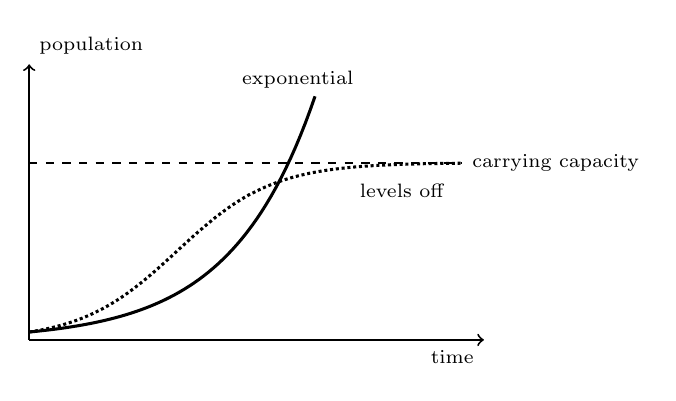
\begin{tikzpicture}[font=\small, x=0.55cm, y=0.5cm]
  \draw[->, line width=0.7pt] (0,0) -- (10.5,0) node[below left, font=\scriptsize] {time};
  \draw[->, line width=0.7pt] (0,0) -- (0,7) node[above right, font=\scriptsize] {population};
  \draw[line width=1.1pt, domain=0:6.6, samples=60] plot (\x, {0.2*exp(0.52*\x)});
  \node[font=\scriptsize] at (6.2,6.6) {exponential};
  \draw[dashed, line width=0.6pt] (0,4.5) -- (10,4.5) node[right, font=\scriptsize] {carrying capacity};
  \draw[line width=1.1pt, densely dotted, domain=0:10, samples=80] plot (\x, {4.5/(1+21.5*exp(-0.9*\x))});
  \node[font=\scriptsize] at (8.6,3.8) {levels off};
\end{tikzpicture}
\figcap{With no limits a population grows faster and faster (solid). Limiting factors make it level off at the carrying capacity (dotted).}
\end{center}

\begin{workedex}{Doubling}
24 rabbits double every year. How many after 10 years, with no limits?

\smallskip
$24 \times 2^{10} = 24 \times 1024 = \mathbf{24\,576}$ rabbits. After 20 years it would be over 25 million.
\end{workedex}

\begin{wedo}{Doubling}
A population of 100 cane toads doubles every two years. How many toads after 10 years? Why will the real number eventually stop growing?
\workbox{5cm}
\end{wedo}

\subsection{Saving Small Populations}\label{sub:a7.2}

\begin{workedex}{Why one big reserve is not enough}
All the remaining animals of a threatened species live in one reserve. Why is this risky, even if the reserve is protected?

\smallskip
One bushfire, flood or disease outbreak could kill them all at once. The animals cannot mix with others, so inbreeding rises. Recovery plans therefore set up several separate populations, and move animals between them to keep genetic diversity up.
\end{workedex}

\begin{wedo}{Planning genetic rescue}
Eastern barred bandicoots now live in a few fenced reserves and on islands. Explain why managers move bandicoots from one population to another every few years, and one risk of doing so.
\answerbox{5cm}
\end{wedo}

\lessonpart{C}{Practice}{Amber}\label{prac:7}

%%PARTD:9%%

%%PARTD:10%%

%%PARTD:11%%

\lessonpart{D}{Challenge}{Violet}\label{ext:7}

\task An imaginary lizard, the ridge skink, survives in two patches of grassland: 250 skinks in one, 50 in the other, 5\,km apart, with farmland between. Foxes, cats and an uncontrolled weed are spreading. Write a recovery plan with three actions. For each, say which threat it deals with and how you would measure whether it is working.
\answerbox{9cm}

\clearpage
